% !TEX root = /media/ueslei/Ueslei_HD/INPE/PCI/Projetos/Guia_COAWST/main.tex
\chapterimage{header.jpg}
\chapter{Building the ROMS}\index{Building the ROMS}
\bigskip

Before generating the ROMS files, it is necessary to install the libraries and modules. 
In this chapter, we address how to download them, as well as the commands in the terminal to install through \textit{apt-get}.
\bigskip

In this guide we will install the ROMS forcing files programs using Anaconda and Pip. 
Anaconda is a free and open source platform for Python and R and has a package manager called Conda, which makes easy 
to install the libraries. In this guide, we will present both options. 
\bigskip

\begin{tcolorbox}[enhanced,
  grow to left by   = 0cm,
  grow to right by  = 0cm,
  enlarge top by    = 0cm,
  enlarge bottom by = 0cm,
  tcbox raise base,
  boxrule           = 1.0pt,
  left              = 18mm,
  colframe          = red!50!black,coltext=red!25!black,colback=red!10!white,
  overlay           = {\begin{tcbclipinterior}\fill[red!75!blue!50!white] (frame.south west)
    rectangle node[text=white,font=\sffamily\bfseries\footnotesize,rotate=0] {WARNING} ([xshift=18mm]frame.north west);\end{tcbclipinterior}}]
Although the ROMS model will be executed in the cluster, we will build the forcing files our own computer and then place them in the Kerana.
\end{tcolorbox}
\bigskip

\subsection{Installing Anaconda}\label{condasec}
\bigskip
Anaconda\textcolor{bleu_cite}{\textit{}\footnote{\textcolor{bleu_cite}{\href{https://www.anaconda.com/products/individual}{https://www.anaconda.com/products/individual}}}}
is a distribution for Python and R that supports the various libraries and packages used in this guide, 
making installation easier. To install, enter the directory where the installation file is located, change the installation permissions of the file and 
follow the installer's instructions:
\bigskip

\begin{bashcode}
 sudo chmod 770 Anaconda.sh
 ./Anaconda2.sh
\end{bashcode}
\bigskip

Next, enter the following commands on the terminal to install the libraries needed to build a project on ROMS:
\bigskip

\begin{bashcode}
conda install -c mutirri szip
conda install -c anaconda zlib
conda install -c conda-forge udunits
conda install -c anaconda netcdf4
conda install -c conda-forge netcdf-fortran
conda install -c anaconda numpy
conda install -c anaconda scipy
conda install -c conda-forge esmf
conda install -c conda-forge esmpy 
conda install -c conda-forge lpsolve55 
conda install -c conda-forge cftime
conda install -c anaconda basemap 
conda install -c conda-forge basemap-data-hires 
conda install -c conda-forge matplotlib 
\end{bashcode}
\bigskip

\section{Installing Pyroms}\index{Instalando o Pyroms}
\bigskip

\begin{tcolorbox}[enhanced,
    grow to left by   = 0cm,
    grow to right by  = 0cm,
    enlarge top by    = 0cm,
    enlarge bottom by = 0cm,
    tcbox raise base,
    boxrule           = 1.0pt,
    left              = 18mm,
    colframe          = red!50!black,coltext=red!25!black,colback=red!10!white,
    overlay           = {\begin{tcbclipinterior}\fill[red!75!blue!50!white] (frame.south west)
      rectangle node[text=white,font=\sffamily\bfseries\footnotesize,rotate=0] {WARNING} ([xshift=18mm]frame.north west);\end{tcbclipinterior}}]
Pyroms was recently updated and is working only with Python3. We suggest to install Python3 with Anaconda since Python2 will no longer be updated after 01 January 2020.
  \end{tcolorbox}
\bigskip

This section will show you how to install Pyroms. It is a collection of tools to create ROMS files originally started by Rob Hetland as a
project on Google Code and rewritten by Frederic Castruccio.
\bigskip

Pyhon3 can be easily installed using Pip, a command line tool that allows you to install software packages written in Python.
\bigskip

\begin{bashcode}
sudo apt install python3-pip
\end{bashcode}
\bigskip

Install Git to access the Pyroms repository:\label{gitinfo}
\bigskip

\begin{bashcode}
sudo apt-get install git
\end{bashcode}
\bigskip

Then, download the Pyroms by cloning the repository at Github:
\bigskip

\begin{bashcode}
git clone https://github.com/ESMG/pyroms.git
\end{bashcode}
\bigskip

Enter inside the Pyroms folder and install it using Pip:
\bigskip

\begin{bashcode}
pip install -e pyroms/pyroms
pip install -e pyroms/pyroms_toolbox
pip install -e pyroms/bathy_smoother
\end{bashcode}
\bigskip

This will install both three Pyroms packages, but if you try to import any of then without \textit{Scrip} installed, you will get a warning 
similar to that found in \textcolor{bleu_cite}{Figure \ref{scriperror}}:
\bigskip

\begin{figure}[H]
  \centering
  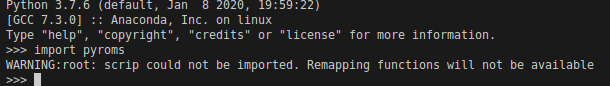
\includegraphics[width=0.85\textwidth]{scriperror.png}
  \caption{Scrip warning when Pyroms is imported without installing it.}
  \label{scriperror}
\end{figure}
\bigskip

As stated in the Pyroms repository, the scrip module is not available via Conda or any other package repository, but it can be built 
and installed as the following:
\bigskip

\begin{bashcode}
cd pyroms/pyroms/external/scrip/source/
\end{bashcode}
\bigskip

Then, print the active Conda environment path. This will be used to find the netCDF library.
\bigskip

\begin{bashcode}
conda info | grep "active env location"
\end{bashcode}
\bigskip

The output must be something like as the following:
\bigskip

\begin{bashcode}
active env location : /home/USER/anaconda3
\end{bashcode}
\bigskip

Export the PREFIX variable with the location found in the previous step.
\bigskip

\begin{bashcode}
export PREFIX=/home/USER/anaconda3
\end{bashcode}
\bigskip

Install the module with the make command.
\bigskip

\begin{bashcode}
sudo make DEVELOP=1 PREFIX=$PREFIX install
\end{bashcode}
\bigskip

Move the Scrip files to the Pyroms folder, like the following:
\bigskip

\begin{bashcode}
  mv -vf scrip*.so ../../../pyroms
\end{bashcode}
\bigskip


\subsection{Pyroms Palau\_Hycom test case}\index{O model2roms}\label{pyromstest}
\bigskip

\begin{tcolorbox}[enhanced,
    grow to left by   = 0cm,
    grow to right by  = 0cm,
    enlarge top by    = 0cm,
    enlarge bottom by = 0cm,
    tcbox raise base,
    boxrule           = 1.0pt,
    left              = 18mm,
    colframe          = red!50!black,coltext=red!25!black,colback=red!10!white,
    overlay           = {\begin{tcbclipinterior}\fill[red!75!blue!50!white] (frame.south west)
      rectangle node[text=white,font=\sffamily\bfseries\footnotesize,rotate=0] {WARNING} ([xshift=18mm]frame.north west);\end{tcbclipinterior}}]
This section will present the script files used by Pyroms as example to create ROMS forcing files. If you want to used our model2roms toolbox, check Section \textcolor{bleu_cite}{\ref{model2romssec}}.
  \end{tcolorbox}
\bigskip

\textbf{This subsection was written by Dr. Jonas Takeo Carvalho.  \newline Lattes CV: \textit{\textcolor{bleu_cite}{\href{http://lattes.cnpq.br/8827254187143196}{http://lattes.cnpq.br/8827254187143196}}}} 
\bigskip

You can check several examples inside the \textit{examples} folder in Pyroms root directory. In this section 
we will show how to run the Palau\_Hycom test case. Before running the scripts, check the paths contained within its structure. 
In some scripts it is necessary to change the indicated path to the path in which your files are. First, run the file \textit{get\_hycom\_GLBa0.08\_Palau\_grid.py}
to create the grid named \textit{HYCOM\_GLBa0.08\_Palau\_grid.nc}. This is a grid that represents Hycom data.
\bigskip

\begin{bashcode}
python get_hycom_GLBa0.08_Palau_grid.py
\end{bashcode}
\bigskip

Next, download the temperature, salinity, \textit{u} and \textit{v} components of the currents and SSH variables 
through the scripts for this data. Each variable has a script. In the example for this tutorial, in addition to the paths within the scripts, the number of days 
to download was also modified. On lines 79 and 82 of each variable file (for example, \textbf{get\_hycom\_GLBa0.08\_Palau\_temp\_2015.py} the values \textit{366} and
365 were changed to 1 (it means that it will be downloaded only one day). Before running, create a directory called \textit{data}. The downloaded files will be placed in
this directory.
\bigskip

\subsubsection{Manipulating the files}
\bigskip

After executing the grid generation and data download script files, you will have the following files:
\bigskip

\begin{itemize}
    \item HYCOM\_GLBa0.08\_PALAU\_grid.nc
    \item HYCOM\_GLBa0.08\_temp\_2015\_001.nc
    \item HYCOM\_GLBa0.08\_salt\_2015\_001.nc
    \item HYCOM\_GLBa0.08\_ssh\_2015\_001.nc   
    \item HYCOM\_GLBa0.08\_u\_2015\_001.nc
    \item HYCOM\_GLBa0.08\_v\_2015\_001.nc    
\end{itemize}
\bigskip

We must now create the initial and boundary conditions with the downloaded data, but first we must concatenate them into a single file. 
As they are files with different variables, without a common variable, we must first generate a variable to be shared between them, and still, be useful 
for reading the ROMS model. Then the variable \textit{ocean\_time} will be created, which is read by the model and common to all files.
For the most recent data from Hycom, this variable already exists, but but for older Hycom data, this step is important. Use \textit{NCO} to do this step:
\bigskip

\begin{itemize}
    \item ncks -O  $-$$-$mk\_rec\_dmn ocean\_time HYCOM\_GLBa0.08\_ssh\_2015\_001.nc  var1.nc
    \item ncks -O $-$$-$mk\_rec\_dmn ocean\_time HYCOM\_GLBa0.08\_salt\_2015\_001.nc  var2.nc
    \item ncks -O $-$$-$mk\_rec\_dmn ocean\_time HYCOM\_GLBa0.08\_temp\_2015\_001.nc  var3.nc    
    \item ncks -O $-$$-$mk\_rec\_dmn ocean\_time HYCOM\_GLBa0.08\_u\_2015\_001.nc  var4.nc
    \item ncks -O $-$$-$mk\_rec\_dmn ocean\_time HYCOM\_GLBa0.08\_v\_2015\_001.nc  var5.nc  
\end{itemize}
\bigskip

After including the variable \textit{ocean\_time}, concatenate the files into a single file with the commands: 
\bigskip

\begin{itemize}
    \item ncks  -a  -O var1.nc  HYCOM\_GLBa0.08\_2015\_001.nc
    \item ncks  -a  -A var2.nc  HYCOM\_GLBa0.08\_2015\_001.nc
    \item ncks  -a  -A var3.nc  HYCOM\_GLBa0.08\_2015\_001.nc
    \item ncks  -a  -A var4.nc  HYCOM\_GLBa0.08\_2015\_001.nc
    \item ncks  -a  -A var5.nc  HYCOM\_GLBa0.08\_2015\_001.nc
\end{itemize}
\bigskip

The file \textit{HYCOM\_GLBa0.08\_2015\_001.nc} contains all 5 variables necessary to generate boundary and initial conditions.
Now, change the paths in the scripts \textit{make\_bdry\_file.py} and \textbf{make\_ic\_file.py} pointing to the local directories you are using. 
It is also necessary to do the same thing for interpolation script files. All files with the initial name \textit{remap} must be updated with you path.
\bigskip

After all the paths have been corrected, first run the script \textit{make\_remap\_weights\_file.py}, which will generate the files 
used during the process of creating the initial and boundary condition files. After these files are generated, execute the scripts \textit{make\_bdry\_file.py} and
\textbf{make\_ic\_file.py} remembering only to add the year you chosed on the command line, for example: 
\bigskip

\begin{bashcode}
python make_bdry_file.py 2015
\end{bashcode}
\bigskip
    
Should be generated the files \textit{HYCOM\_GLBy0.08\_2019\_001\_ic\_PALAU.nc} and \textit{HYCOM\_GLBy0.08\_2019\_001\_bdry\_PALAU.nc}
\bigskip

\subsubsection{Observations}
\bigskip

Pyroms uses a file called \textit{gridid.txt}, which contains information regarding the ROMS grid, such as the name of the grid, the number of 
vertical levels, among other parameters. This file can be found in Pyroms in the \textit{pyroms/examples} directory. We should note that the information in 
the PALAU grid is already in the file, but it is necessary to change the directory path.
\bigskip

Another information that we must take into account is that this grid generated for PALAU is not a typical ROMS grid, it is only to be 
an example. The \textit{gridid.txt} file must contain the information from the ROMS notes, which will also be used to make the model, so we must 
export this file to be viewed in any directory, as an example.
\bigskip

In addition to this command, it is recommended to export in your \textit{.bashrc} file the paths of the Python environment created for Pyroms: 
\bigskip

\begin{bashcode}[fontsize=\scriptsize]
    export PATH="$HOME/install/anaconda3/bin:\$PATH"
    export PYTHONPATH=\$PYTHONPATH:$HOME/install/anaconda3/envs/pyroms37/lib
    export PYTHONPATH=\$PYTHONPATH:$HOME/install/anaconda3/envs/pyroms37/lib/python3.7/site-packages
\end{bashcode}
\bigskip

\subsection{Pyroms LOA-Antarctica test case}\index{O model2roms}\label{loatest}
\bigskip

\begin{tcolorbox}[enhanced,
    grow to left by   = 0cm,
    grow to right by  = 0cm,
    enlarge top by    = 0cm,
    enlarge bottom by = 0cm,
    tcbox raise base,
    boxrule           = 1.0pt,
    left              = 18mm,
    colframe          = red!50!black,coltext=red!25!black,colback=red!10!white,
    overlay           = {\begin{tcbclipinterior}\fill[red!75!blue!50!white] (frame.south west)
      rectangle node[text=white,font=\sffamily\bfseries\footnotesize,rotate=0] {WARNING} ([xshift=18mm]frame.north west);\end{tcbclipinterior}}]
This section will present the script files used by Pyroms as example to create ROMS forcing files. If you want to used our model2roms toolbox, check Section \textcolor{bleu_cite}{\ref{model2romssec}}.
  \end{tcolorbox}
\bigskip

\textbf{This subsection was written by Dr. Jonas Takeo Carvalho.  \newline Lattes CV: \textit{\textcolor{bleu_cite}{\href{http://lattes.cnpq.br/8827254187143196}{http://lattes.cnpq.br/8827254187143196}}}} 
\bigskip

Based on the structure of the Palau test case, the scripts to generate initial and boundary conditions with Pyroms were replicated to the Antarctica region. 
We selected the Antarctic Peninsula as its central point in the grid. Below are some steps to generate the desired files.
\bigskip

\subsubsection{Replicating the scripts}
\bigskip

In addition to replicating the scripts to generate the grid that represents and download Hycom data, we must generate the ROMS grid for the region of interest.
 We can use as an example the script \textit{make\_YELLOW\_grd\_v1.py} of the Yellow\_Sea test case. In this script we must replace the name, longitude and latitude values, 
 grid dimensions, and vertical coordinate values. For this case, the ROMS grid, and its information from the \textit{gridid.txt} file can be found in the 
 Kerana's repository. 
\bigskip

In the script files for downloading the data (\textit{get\_hycom\_GLBa0.08\_variable.py}), it is also necessary to change the path of the Hycom data to be 
downloaded. In the Palau example, the structure of the download data is from 2015. This structure is changed for periods called \textit{exp}. These scripts are also 
found in the repository.
\bigskip

\subsubsection{Correcting dimensions}
\bigskip

A necessary change in the scripts is the grid size that represents Hycom and its downloaded data. After defining the limits for both latitude and longitude,
we must choose an additional number of points outside the grid. If we don't define any extra points in the grid or in the data, the following error will be displayed:
\bigskip

\begin{bashcode}[fontsize=\scriptsize]
ValueError: operands could not be broadcast together with shapes (873,1249) (875,1251)
\end{bashcode}
\bigskip

The first set refers to the size of the grid that represents the Hycom and the second set represents the downloaded Hycom data. We must adjust these values, 
increasing the dimension of the latitude, longitude and variable within the Hycom data download scripts by 2 units compared to the script representing the Hycom grid. 
In the figure \textcolor{bleu_cite}{\ref{hycomantartic1}} and in the figure \textcolor{bleu_cite}{\ref{hycomantartic2}} we can see the location in the scripts where this addition is made.
\bigskip

\begin{figure}[H]
    \centering
    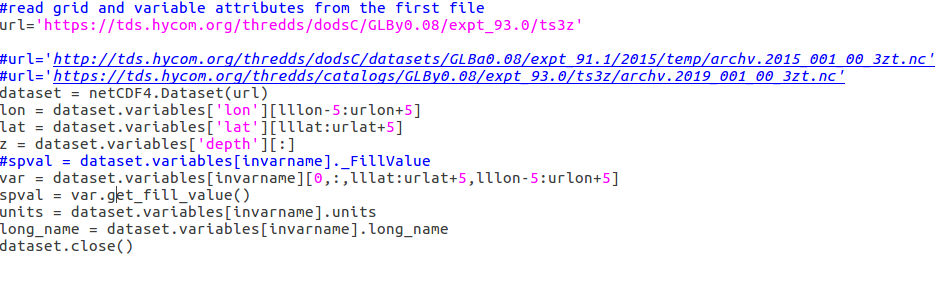
\includegraphics[width=0.85\textwidth]{gridHycom.png}
    \caption{\textbf{get\_hycom\_GLBa0.08\_antartic\_grid.py script}}
    \label{hycomantartic1}
\end{figure}
\bigskip

\begin{figure}[H]
    \centering
    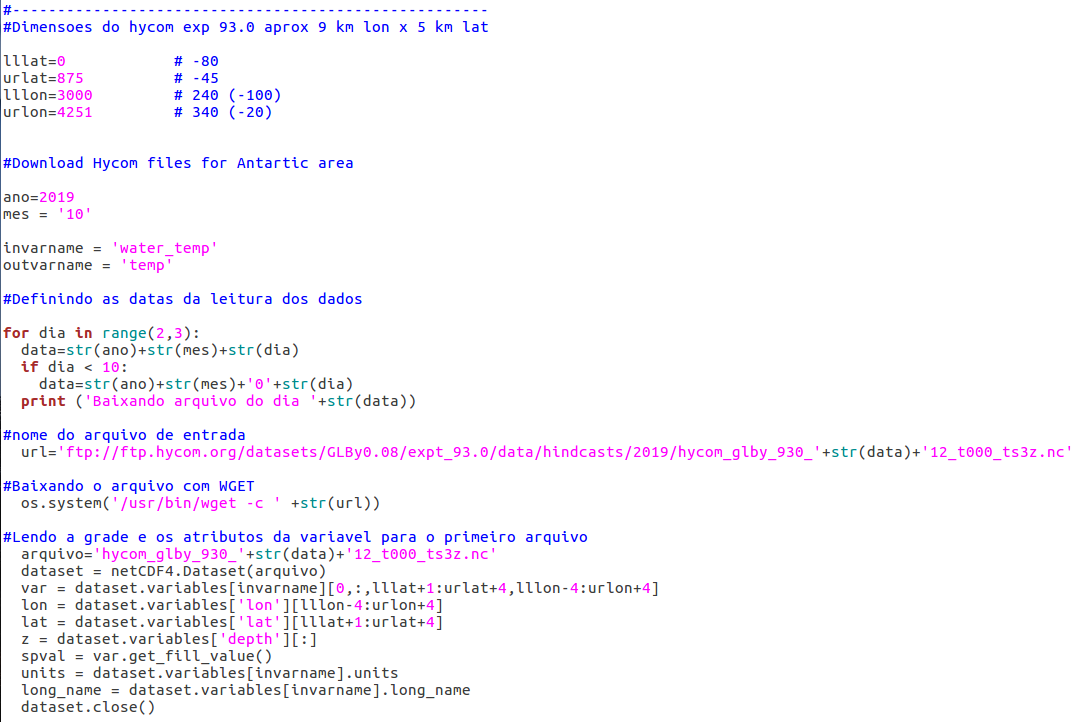
\includegraphics[width=0.85\textwidth]{dadosHycom.png}
    \caption{\textbf{get\_hycom\_GLBa0.08\_antartic\_temp.py script}}
    \label{hycomantartic2}
\end{figure}
\bigskip

Note that in the grid script, the minimum and maximum longitude receive +5 and -5 extra values. In the download data script file, the minimum and maximum
longitude receive -4 and +4 extra value, solving the ValueError. These values worked well in the Antartic grid. This exercise does not have a specific rule, it is 
necessary to start from a value of your desire and observe the obtained results.
\bigskip

When checking the initial and countour files, it should be noted that the edges are with the correct values. If any of the edges have extreme or zero values
where they should have valid values, you must redo the files by testng other extra value for longitude and latitude. The initial condition file, if it is wrong, will also 
present extreme values, and an unusual pattern for the region. 
\bigskip

When generating a long-term series, check if there is any missing day from the sries, ai it will generate zero values for this day and when running the model,
it wil l propably interrupt the simulation.  The initial and boundary condition files should look similar to the figures \textcolor{bleu_cite}{\ref{hycomantartic3}} and \textcolor{bleu_cite}{\ref{hycomantartic4}}.
\bigskip


\begin{figure} [!htb] 
    \centering
    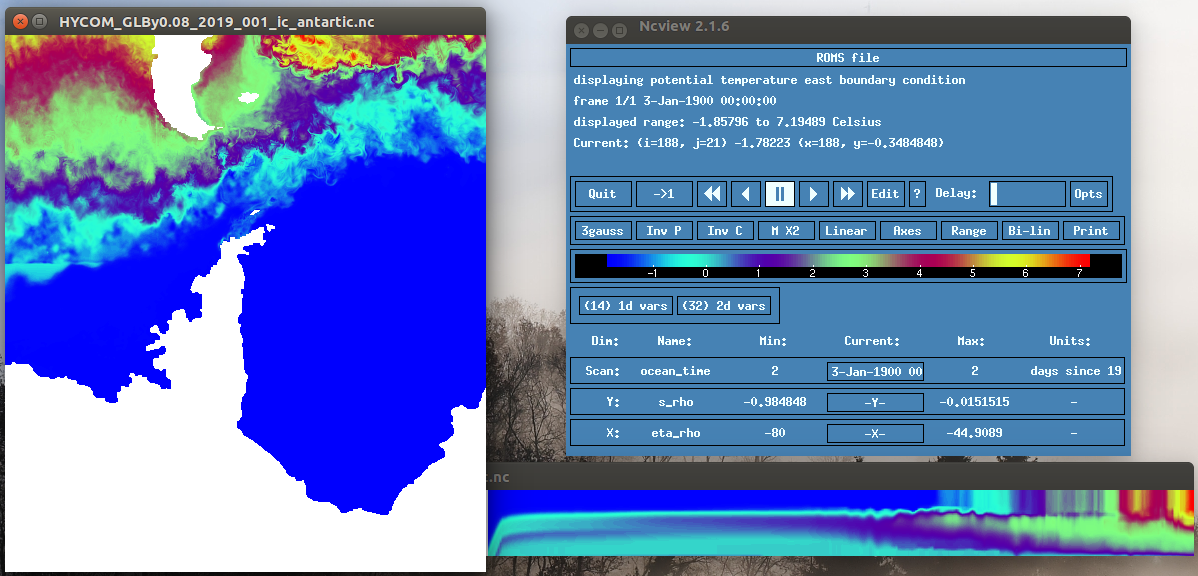
\includegraphics[trim=0.15cm 0.15cm 0.15cm 0.5cm,clip,width=0.9\textwidth]{temperatura.png}
    \caption{Initial condition and east temperature boundary.}
    \label{hycomantartic3}
    \end{figure}
    
    
    
    %Figura5
    \begin{figure} [!htb] 
    \centering
    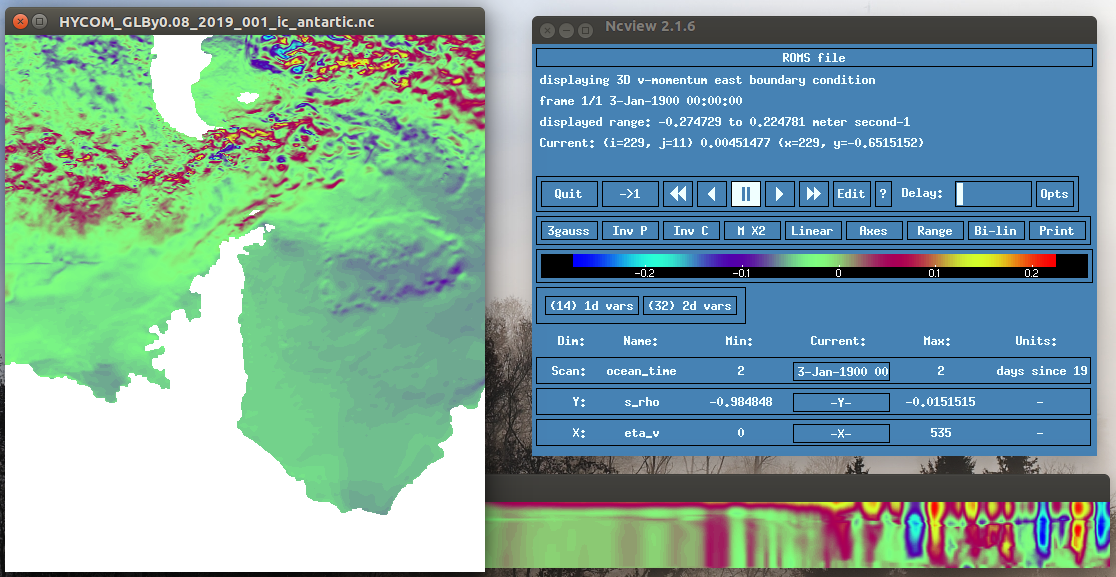
\includegraphics[trim=0.15cm 0.15cm 0.15cm 0.5cm,clip,width=0.9\textwidth]{compV.png}
    \caption{Initial condition and east boundary of the current \textit{v} component.}
    \label{hycomantartic4}
    \end{figure}
\bigskip

\section{The model2roms toolbox}\index{O model2roms}\label{model2romssec}
\bigskip

In this section, you will be introduced to install model2roms, the toolbox used to generate ROMS forcing files and its grid. 
It was created and is being updated by Trond Kristiansen (\textcolor{bleu_cite}{\cite{Trond2019}}) and we adapted to the needs of 
LOA-INPE. 
\bigskip

To download \textit{model2roms}, enter in your \textit{home} folder and download using Github:
\bigskip

\begin{tcolorbox}[enhanced,
    grow to left by   = 0cm,
    grow to right by  = 0cm,
    enlarge top by    = 0cm,
    enlarge bottom by = 0cm,
    tcbox raise base,
    boxrule           = 1.0pt,
    left              = 18mm,
    colframe          = green!50!black,coltext=green!25!black,colback=green!10!white,
    overlay           = {\begin{tcbclipinterior}\fill[green!75!blue!50!white] (frame.south west)
      rectangle node[text=white,font=\sffamily\bfseries\footnotesize,rotate=0] {NOTE} ([xshift=18mm]frame.north west);\end{tcbclipinterior}}]
Read how to install Git in the subsection \textcolor{bleu_cite}{\ref{gitinfo}}.
  \end{tcolorbox}
\bigskip

\begin{bashcode}
cd $HOME
git clone https://github.com/usutil/model2roms
\end{bashcode}
\bigskip

Change the folder name from \textit{model2roms-master} to \textit{model2roms}:
\bigskip

\begin{bashcode}
mv model2roms-master model2roms
\end{bashcode}
\bigskip

\subsection{Introduction to the ROMS grid}\index{Gerar a grade do ROMS}
\bigskip

To generate the ROMS grid, we will use the code \textit{make\_roms\_grid.py}, located in the \textit{model2roms/grid} 
directory. The code supports the SRTM30\_plus data (\cite{Becker2009}), however, for practical purposes, we will exemplify 
only the data from ETOPO1 (\cite{Amante2009}), which will be discussed in the next subsection.
\bigskip

Install basemap to use the code, if you have not previously installed.
\bigskip

\begin{bashcode}
conda install -c anaconda basemap
\end{bashcode}
\bigskip

\subsection{ETOPO1 1 Arc-Minute Global Relief Model}\index{O ETOPO1 1 Arc-Minute Global Relief Model}
\bigskip

The ETOPO1\textcolor{bleu_cite}{\textit{}\footnote{\textcolor{bleu_cite}{\href{https://www.ngdc.noaa.gov/mgg/global/global.html}{https://www.ngdc.noaa.gov/mgg/global/global.html}}}}
 (\cite{Amante2009}; Figure \textcolor{bleu_cite}{\ref{etopo1}}) 
is produced by the National Geophysical Data Center and provides two layers of relief information.
The layers include bathymetry over the oceans and some of the main lakes on Earth.
 Terrestrial topography and ocean bathymetry are based on SRTM30 topography and through various bathymetric cruises.
\bigskip

Visit the site
and subset your area of interest on the ETOPO1 website map and download the data in NetCDF format.

\bigskip  
   
\begin{figure}[H]
    \centering
    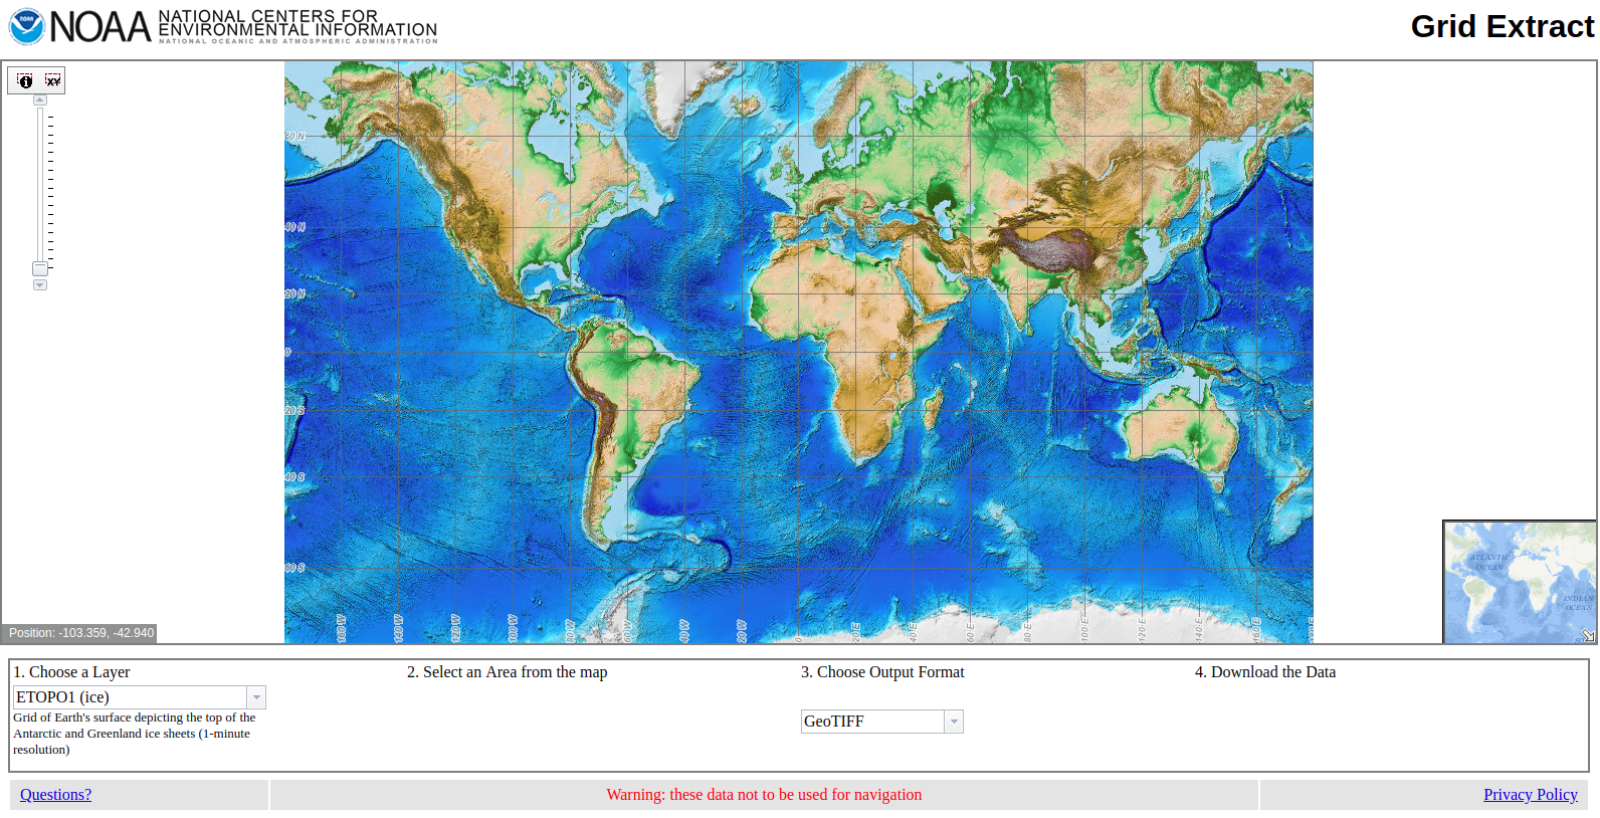
\includegraphics[width=0.85\textwidth]{etopo1.png}
    \caption{ETOPO1 webpage.}
    \label{etopo1}
\end{figure}
\bigskip


\bigskip

\begin{tcolorbox}[enhanced,
    grow to left by   = 0cm,
    grow to right by  = 0cm,
    enlarge top by    = 0cm,
    enlarge bottom by = 0cm,
    tcbox raise base,
    boxrule           = 1.0pt,
    left              = 18mm,
    colframe          = red!50!black,coltext=red!25!black,colback=red!10!white,
    overlay           = {\begin{tcbclipinterior}\fill[red!75!blue!50!white] (frame.south west)
      rectangle node[text=white,font=\sffamily\bfseries\footnotesize,rotate=0] {WARNING} ([xshift=18mm]frame.north west);\end{tcbclipinterior}}]
The script \textit{make\_roms\_grid.py} does not allow the selection of the latitude and longitude limits of the grid, therefore, be as accurate as possible when subseting of your area.

\end{tcolorbox}
\bigskip

\subsubsection{Creating the ROMS grid}\index{Gerando a grade do ROMS}
\bigskip

Enter the \textit{model2roms} directory and look for the \textit{grid} subfolder. Open the code \textit{make\_roms\_grid.py}.
\bigskip

\begin{bashcode}
cd $HOME/model2roms/grid
gedit make_roms_grid.py
\end{bashcode}
\bigskip

As Figure \textcolor{bleu_cite}{\ref{fazgrade}} shown, the variables that will be modified are:
\bigskip

\begin{itemize}
\item \textbf{grd\_name}: Grid name;
\item \textbf{grd\_final}: The NetCDF file name of the grid;
\item \textbf{etopo1\_dir}: The directory where the ETOPO1 NetCDF file is located;
\item\textbf{srtm\_dir}: The directory where the SRTM\_30\_PLUS NetCDF file is located; 
\item \textbf{hmin}: Value of \textit{h} parameter;
\item \textbf{theta\_b}: Control parameter for coordinates close to the ocean floor;
\item \textbf{theta\_s}: Control parameter for coordinates close to the surface;
\item \textbf{Tcline}: Critical depth, in meters, controlling the elongation of the coordinates following the terrain. It can be interpreted as the width of the surface where vertical resolution is best;
\item \textbf{N}: Number of Sigma layers;
\item \textbf{rmax}: Topography smoothing factor;
\item \textbf{intrp\_method}: Grid interpolation method: Linear (\textit{linear}) or Near Neighbor (\textit{nn});
\item \textbf{grid\_resolution}: Grid resolution;
\item\textbf{max\_depth}: Maximum grid depth.
\end{itemize}
\bigskip

\begin{tcolorbox}[enhanced,
    grow to left by   = 0cm,
    grow to right by  = 0cm,
    enlarge top by    = 0cm,
    enlarge bottom by = 0cm,
    tcbox raise base,
    boxrule           = 1.0pt,
    left              = 18mm,
    colframe          = red!50!black,coltext=red!25!black,colback=red!10!white,
    overlay           = {\begin{tcbclipinterior}\fill[red!75!blue!50!white] (frame.south west)
      rectangle node[text=white,font=\sffamily\bfseries\footnotesize,rotate=0] {WARNING} ([xshift=18mm]frame.north west);\end{tcbclipinterior}}]
      In \textit{grid\_resolution}, it is necessary to place the numerator to do the ETOPO1 calculation. For example: as ETOPO1 has 1/60° of spatial resolution, if the chosen spatial resolution is 1/12°, the value of \textit{grid\_resolution} will be 5, because 5/60° is the same as 1/12° .\end{tcolorbox}
\bigskip

\begin{tcolorbox}[enhanced,
    grow to left by   = 0cm,
    grow to right by  = 0cm,
    enlarge top by    = 0cm,
    enlarge bottom by = 0cm,
    tcbox raise base,
    boxrule           = 1.0pt,
    left              = 18mm,
    colframe          = yellow!50!black,coltext=yellow!25!black,colback=yellow!10!white,
    overlay           = {\begin{tcbclipinterior}\fill[yellow!75!blue!50!white] (frame.south west)
      rectangle node[text=white,font=\sffamily\bfseries\footnotesize,rotate=0] {ATTENTION} ([xshift=18mm]frame.north west);\end{tcbclipinterior}}]
As we do not use the data from SRTM\_30\_PLUS, the variable \textit{srtm\_dir} does not need to be modified.
\end{tcolorbox}
\bigskip

\begin{figure}[H]
    \centering
    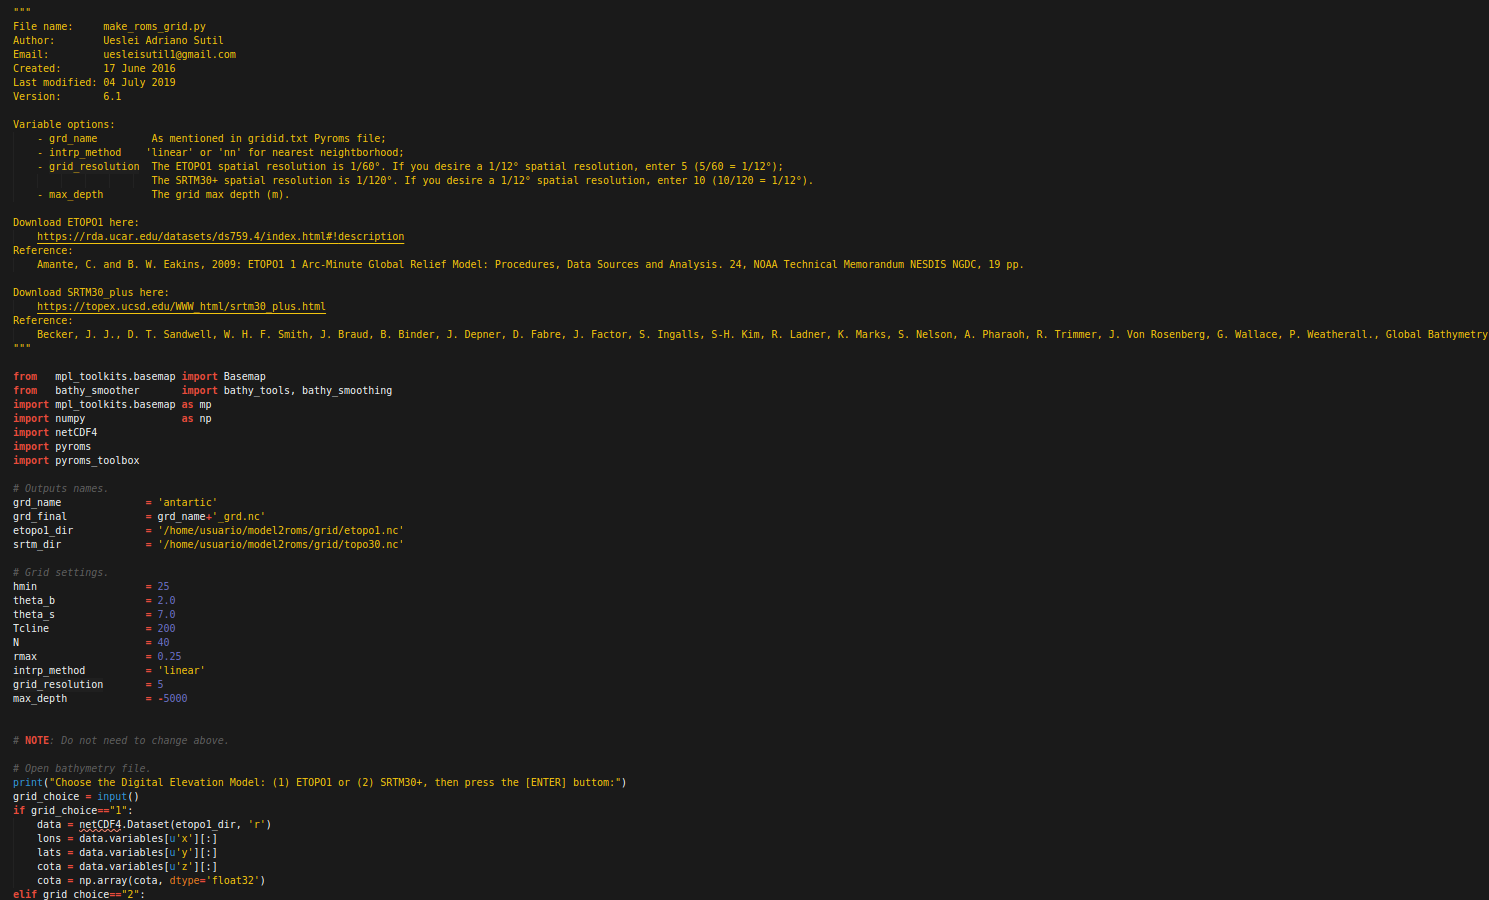
\includegraphics[width=1\textwidth]{makegrid.png}
    \caption{Screenshot of the \textit{make\_grid.py} file, which is located in the \textit{model2roms/grid} folder.}
    \label{fazgrade}
\end{figure}
\bigskip

After making the changes, just run the code. Type it:
\bigskip

\begin{bashcode}
ipython make_roms_grid.py --pylab
\end{bashcode}
\bigskip

\subsection{Gridbuilder}
\bigskip

Optionally, you can use the Gridbuilder\textcolor{bleu_cite}{\textit{}\footnote{\textcolor{bleu_cite}{\href{https://austides.com/wp-content/uploads/GridBuilder-v0.99.pdf}{https://austides.com/wp-content/uploads/GridBuilder-v0.99.pdf}}}}.
It is a tool that can be an alternative to build the grid used in the oceanic model instead of using the \textit{make\_grid.py} script. It is is intended for rapid development of grids for numerical ocean models
with a particular emphasis on elements commonly used in ROMS. The website offers a PDF with valuable informations about how to use the program.

\subsection{Introduction to ROMS forcing files}\index{Introdução sobre as condições do ROMS}
\bigskip

We will use \textit{model2roms} to generate the ROMS conditions. The toolbox supports data from GLORYS12V1 (\cite{Fernandez2018}) 
and SODA3 (\cite{Carton2018}), however, we will only use GLORYS12V1 as an example.

\subsection{Global Ocean Physics Reanalysis (GLORYS)}\index{O Global Ocean Physics Reanalysis (GLORYS)}
\bigskip

GLORYS\textcolor{bleu_cite}{\textit{}\footnote{\textcolor{bleu_cite}{\href{http://marine.copernicus.eu/services-portfolio/access-to-products/?option=com\_csw\&view=details\&product\_id=GLOBAL\_REANALYSIS\_PHY\_001\_030}{\nolinkurl{http://marine.copernicus.eu/services-portfolio/access-to-products/?option=com\_csw\&view=details\&product\_id=GLOBAL\_REANALYSIS\_PHY\_001\_030}}}}}
is a global reanalysis of the ocean with a 1/12° spatial resolution with daily and monthly temporal resolution and 
50 vertical levels. It is based on the current CMEMS global weather forecasting system and is forced by ECMWF's ERA-Interim from the NEMO model.
A Kalman filter with reduced order is used to assimilate the sea altimetry, sea surface temperature, sea ice concentration data obtained 
from remote sensing and the \textit{in situ} data of vertical temperature and salinity profiles .
In addition, a 3D-VAR scheme provides a correction for temperature and salinity deviations.
\bigskip

You can download the GLORYS data using the \textit{download\_glorys\_cmems\_lsl.sh} script provided by Luciana Lima. Go to the repository root folder, download the \textit{download\_glorys\_cmems\_lsl.sh}
file, modify according your needs and execute, as the following:
\bigskip

\begin{bashcode}
cd /scratch/adriano.sutil/repositorio
get download_glorys_cmems_lsl.sh
./download_glorys_cmems_lsl.sh
\end{bashcode}
\bigskip

You can also, download the data manually. But when you try to download, the site will warn you that you will need to create an account.
Register and choose the GLORYS daily data set, as shown in Figure \textcolor{bleu_cite}{\ref{glorys1}}.
\bigskip

\begin{figure}[H]
    \centering
    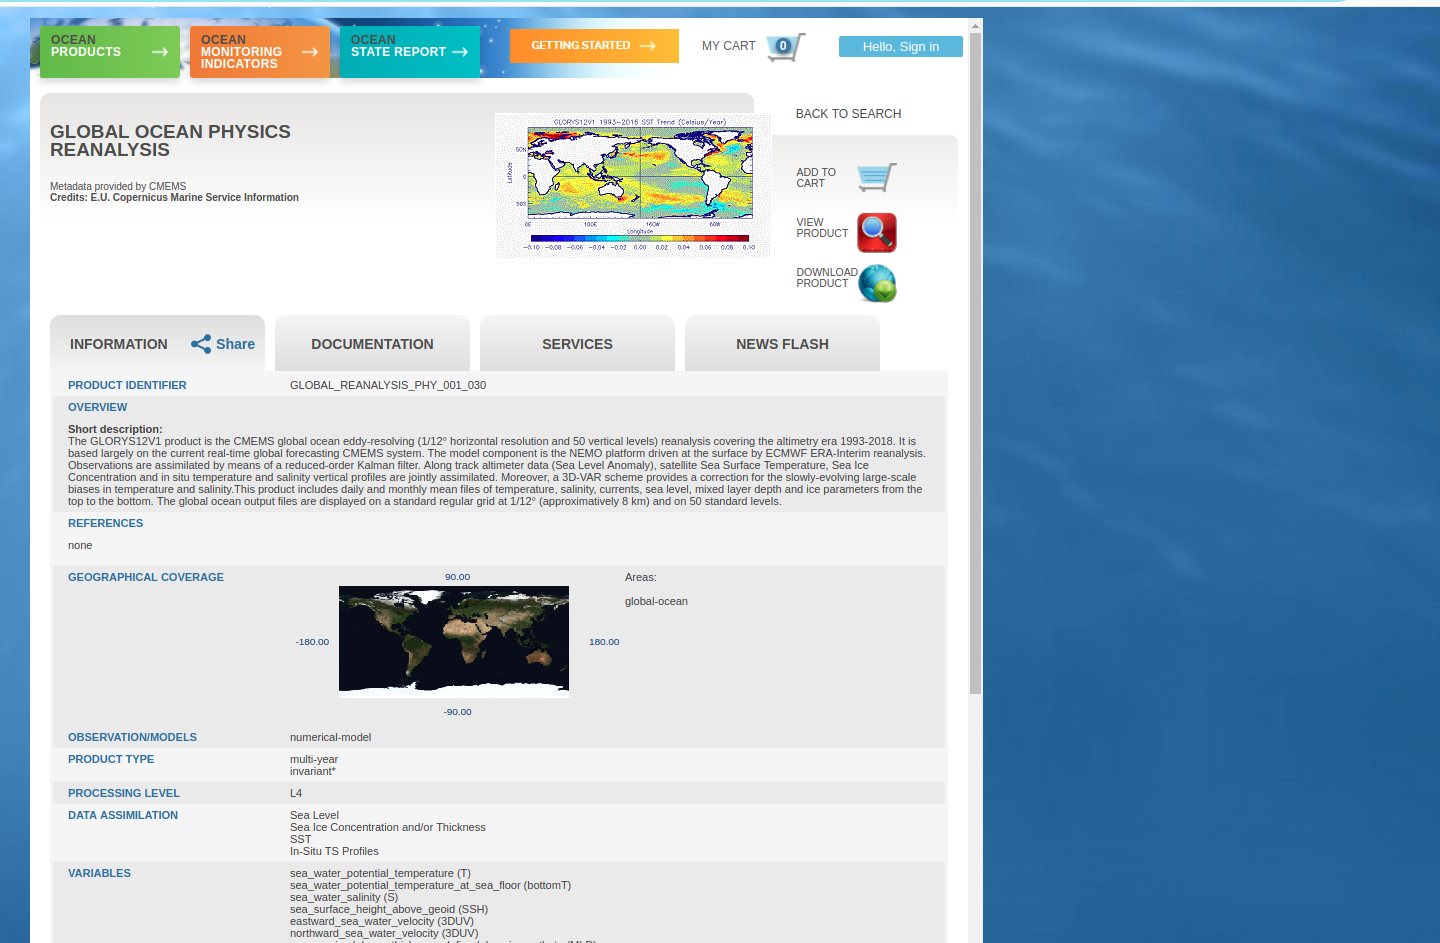
\includegraphics[width=0.7\textwidth]{glorys1.png}
    \caption{Screenshot from GLORYS webpage.}
    \label{glorys1}
\end{figure}
\bigskip

Click on \textit{Dowload product} and, on the next page (Figure \textcolor{bleu_cite}{\ref{glorys2}}), select the area according to 
the latitude and longitude limits of the chosen grid. Also choose the period of data to be downloaded. Also, if you want to use the sea 
ice model in ROMS, select all variables, with the exception of:
\bigskip

\begin{itemize}
    \item \textit{ bottomT - Sea floor potential temperature};
    \item \textit{mlotst - Density ocean mixed layer thickness}.
\end{itemize}
\bigskip

If you choose to not use the sea ice model, do not select the variables:
\bigskip

\begin{itemize}
    \item \textit{siconc - Ice concentration};
    \item \textit{sithick - Sea ice thickness};
    \item \textit{usi - Sea ice eastward velocity};
    \item \textit{vsi - Sea ice northward velocity}.
\end{itemize}
\bigskip

\begin{figure}[H]
    \centering
    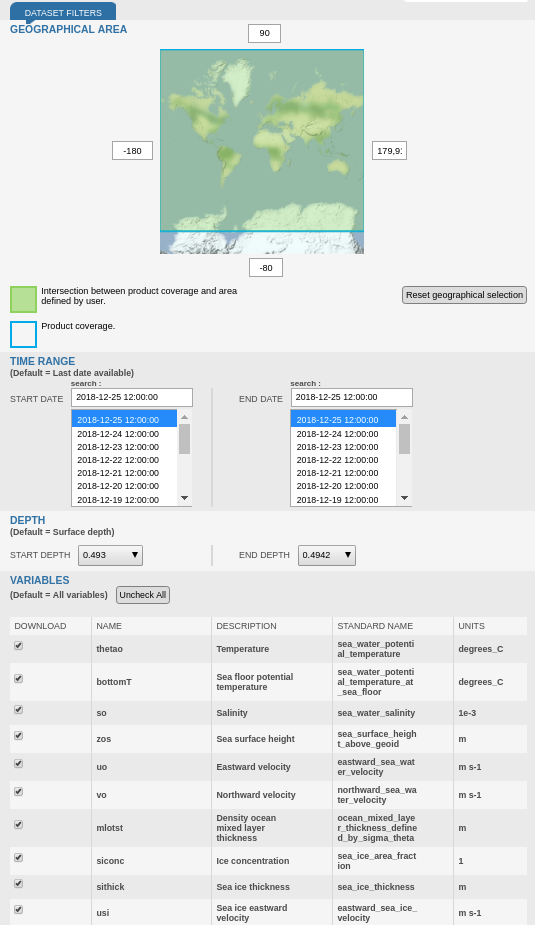
\includegraphics[width=0.5\textwidth]{glorys2.png}
    \caption{Another screenshot from the GLORYS webpage.}
    \label{glorys2}
\end{figure}
\bigskip

The Copernicus server allow download with a maximum size of 1024 mb. 
If the selected period has a larger file size, as for example in Figure \textcolor{bleu_cite}{\ref{glorys3}}, it will be necessary to 
return to the previous step and partition the files into smaller pieces or download the complete set by clicking on \textit{FTP ACCESS}
(Figure \textcolor{bleu_cite}{\ref{glorys3}}).
\bigskip

\begin{figure}[H]
    \centering
    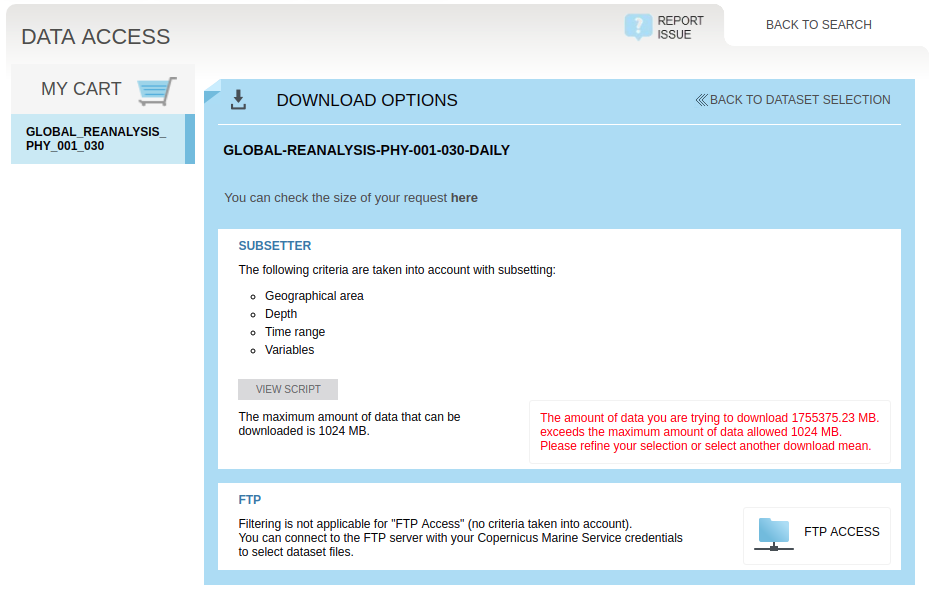
\includegraphics[width=0.6\textwidth]{glorys3.png}
    \caption{Error message when trying to download a text larger than 1024 mb.}
    \label{glorys3}
\end{figure}
\bigskip

If you choose to partition the files or download the files by \textit{FTP}, you will need to create a new file with 
all the concatenated chosen dates. In this case, it is necessary to use \textit{Climate Data Operators} (CDO).
\bigskip

There are two ways to install CDO: by \textit{Conda} or by \textit{apt-get}.
\bigskip

If you choose to use \textit{Conda}, type:
\bigskip

\begin{bashcode}
conda install -c conda-forge cdo
\end{bashcode}
\bigskip

If you choose to use \textit{apt-get}, type:
\bigskip

\begin{bashcode}
sudo apt-get install cdo
\end{bashcode}
\bigskip

After installation, enter the directory where all GLORYS files are located and type:
\bigskip

\begin{bashcode}
cdo cat glorys* glorys.nc
\end{bashcode}
\bigskip

Where: 
\bigskip

\begin{itemize}
    \item  \textit{cdo} means the program command;
    \item \textit{cat} means the concatenation command of all files;
    \item \textit{glorys*} means that all files called \textit{glorys} will be concatenated within the folder;
    \item \textit{glorys.nc} means the final file name created by concatenating with \textit{CDO}.
\end{itemize}
\bigskip

\begin{tcolorbox}[enhanced,
    grow to left by   = 0cm,
    grow to right by  = 0cm,
    enlarge top by    = 0cm,
    enlarge bottom by = 0cm,
    tcbox raise base,
    boxrule           = 1.0pt,
    left              = 18mm,
    colframe          = red!50!black,coltext=red!25!black,colback=red!10!white,
    overlay           = {\begin{tcbclipinterior}\fill[red!75!blue!50!white] (frame.south west)
      rectangle node[text=white,font=\sffamily\bfseries\footnotesize,rotate=0] {WARNING} ([xshift=18mm]frame.north west);\end{tcbclipinterior}}]
Place de dowloaded GLORYS files inside the \textit{\$HOME/model2roms/input} folder.
\end{tcolorbox}

\subsection{Creating ROMS forcing files}\index{Gerando as condições do ROMS}
\bigskip

When opening the \textit{model2roms} folder, it is possible to observe several script files. 
We will start with the file \textit{compile.py}, which will compile the files in Fortran90 to be read by Python. 
\bigskip

Compile the files with the command:
\bigskip

\begin{bashcode}
ipython compile.py --pylab
\end{bashcode}
\bigskip

If your \textit{GLORYS} file name is different from \textit{glorys.nc}, open the code \textit{forcingFilenames.py} 
(Figure \textcolor{bleu_cite}{\ref{forcingfilename}}) and in row 15, change \textit{'glorys.nc'} to the name of the created file.
\bigskip

\begin{bashcode}
cd $HOME/model2roms
gedit forcingFilenames.py
\end{bashcode}
\bigskip

\begin{figure}[H]
    \centering
    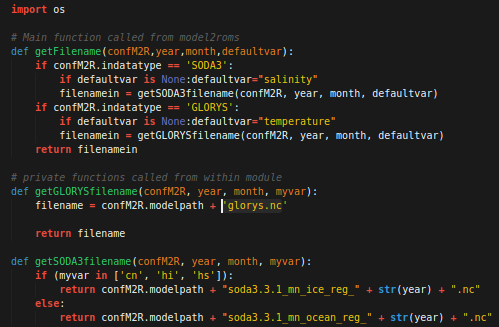
\includegraphics[width=0.6\textwidth]{forcingfilename.png}
    \caption{Screenshot of the \textit{forcingFilename.py} file.}
    \label{forcingfilename}
\end{figure}
\bigskip

Open the file \textit{configM2R.py} and, in row 16 (Figure \textcolor{bleu_cite}{\ref{abrev}}), change the abbreviation \textit{SuaAbreviaçãoAqui} 
to a name of your choice.
\bigskip

\begin{figure}[H]
    \centering
    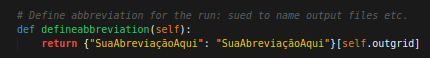
\includegraphics[width=0.6\textwidth]{abrevi.png}
    \caption{Screenshot of the \textit{defineabbreviation} in the code \textit{configM2R.py}.}
    \label{abrev}
\end{figure}
\bigskip

In row 63 (Figure \textcolor{bleu_cite}{\ref{gradediretoriom2r}}), change the grid directory \textit{Minha\_Grade.nc} to your 
grid directory and the abbreviation \textit{SuaAbreviaçãoAqui} by the name chosen in the previous step.
\bigskip

\begin{figure}[H]
    \centering
    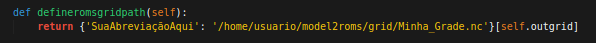
\includegraphics[width=0.6\textwidth]{m2rgriddir.png}
    \caption{Screenshot of the \textit{configM2R.py} code.
    }
    \label{gradediretoriom2r}
\end{figure}
\bigskip

On row 67 (Figure \textcolor{bleu_cite}{\ref{glorysdirm2r}}), change the \textit{GLORYS} file directory to your chosen path.
\bigskip

\begin{figure}[H]
    \centering
    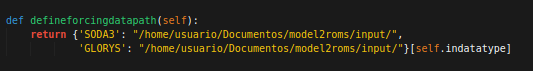
\includegraphics[width=0.6\textwidth]{glorysdirm2r.png}
    \caption{Screenshot of the \textit{configM2R.py} code.}
    \label{glorysdirm2r}
\end{figure}
\bigskip

From row 76 (Figure \textcolor{bleu_cite}{\ref{m2roptions}}), modify according to your project: 
\bigskip

\begin{itemize}
    \item \textbf{self.compileall}: Set as \textit{True} if you want the Fortran files to be recompiled each time \textit{model2roms} is executed;
    \item \textbf{self.createoceanforcing}: Set as \textit{True} to create the hydrodynamic variables;
    \item \textbf{self.createatmosforcing}: Set as \textit{True} to create atmospheric forces. \textbf{Currently this function is in the testing phase and is not entirely available for use};
    \item \textbf{self.writeice}: Set as \textit{True} to create the sea ice variables;
    \item \textbf{self.set2DvarsToZero}: Creates the ice and sea level files with zero values. Since GLORYS has these values, it is recommended to leave it as \textit{False};
    \item \textbf{self.useesmf}: Set as \textit{True} to use \textit{ESMF} to interpolate the GLORYS data to the ROMS grid;
    \item \textbf{self.usefilter}: Set as \textit{True} to apply a filter to smooth out 2D fields.
    \item \textbf{self.myformat}: The extension for writing ROMS input files. It is, by default, \textit{NETCDF};
    \item \textbf{self.timefrequencyofinputdata}: The time frequency of the input data. If using GLORYS, write \textit{day};
    \item \textbf{self.indatatype}: The name of the data used to generate the forcing files. \textit{GLORYS} or \textit{SODA3};
    \item \textbf{self.authorname}: The name of the user using \textit{model2roms};
    \item \textbf{self.authoremail}: The email of the user using \textit{model2roms};
    \item \textbf{self.ingridtype}: It will interpolate the GLORYS grid, which is in \textit{ZLEVEL} coordinate;
    \item \textbf{self.grdtype}: The GLORYS grid type, which is \textit{regular};
    \item \textbf{self.lonname}: The name of the GLORYS longitude variable, which is \textit{longitude};
    \item \textbf{self.latname}: The name of the GLORYS latitude variable, which is \textit{latitude};
    \item \textbf{self.depthname}: The name of the GLORYS depth variable, which is \textit{depth};
    \item \textbf{self.lonname\_u}: The name of the GLORYS U-longitude variable, which is \textit{longitude};
    \item \textbf{self.latname\_u}: The name of the GLORYS U-latitude variable, which is \textit{latitude};
    \item \textbf{self.lonname\_v}: The name of the GLORYS V-longitude variable, which is \textit{longitude};
    \item \textbf{self.latname\_v}: The name of the GLORYS U-latitude variable, which is \textit{latitude};
    \item \textbf{self.timename}: The name of the GLORYS time variable, which is \textit{time};
    \item \textbf{self.realm}: The realm in which \textit{model2roms} is being executed, in this case, \textit{ocean};
    \item \textbf{self.fillvaluein}: The \textit{fillvalue} value of the NetCDF file. By convention, \textit{-1.e20};
    \item \textbf{self.outgrid}: The name of the abbreviation used in the definition \textit{defineabbreviation};
    \item \textbf{self.outgridtype}: If \textit{"ROMS"}, it will create the output in the standard ROMS format;
    \item \textbf{self.nlevels}: The number of vertical levels in the grid. It must be the same as the one chosen in the code \textit{make\_roms\_grid.py};
    \item \textbf{self.vstretching}: It must be the same as the one chosen in the code \textit{make\_roms\_grid.py};
    \item \textbf{self.vtransform}: It must be the same as the one chosen in the code \textit{make\_roms\_grid.py};
    \item \textbf{self.theta\_s}: It must be the same as the one chosen in the code \textit{make\_roms\_grid.py};
    \item \textbf{self.theta\_b}: It must be the same as the one chosen in the code \textit{make\_roms\_grid.py};
    \item \textbf{self.tcline}: It must be the same as the one chosen in the code \textit{make\_roms\_grid.py};   
    \item \textbf{self.hc}: It must be the same as the one chosen in the code \textit{make\_roms\_grid.py};
    \item \textbf{self.start\_year}: The initial year of GLORYS data;
    \item \textbf{self.end\_year}: The final year of GLORYS data;
    \item \textbf{self.start\_month}: The initial month of GLORYS data;
    \item \textbf{self.end\_month}: The final month of GLORYS data;
    \item \textbf{self.start\_day}: The initial day of GLORYS data;
    \item \textbf{self.end\_day}: The final day of GLORYS data;
\end{itemize}
\bigskip

\begin{figure}[H]
    \centering
    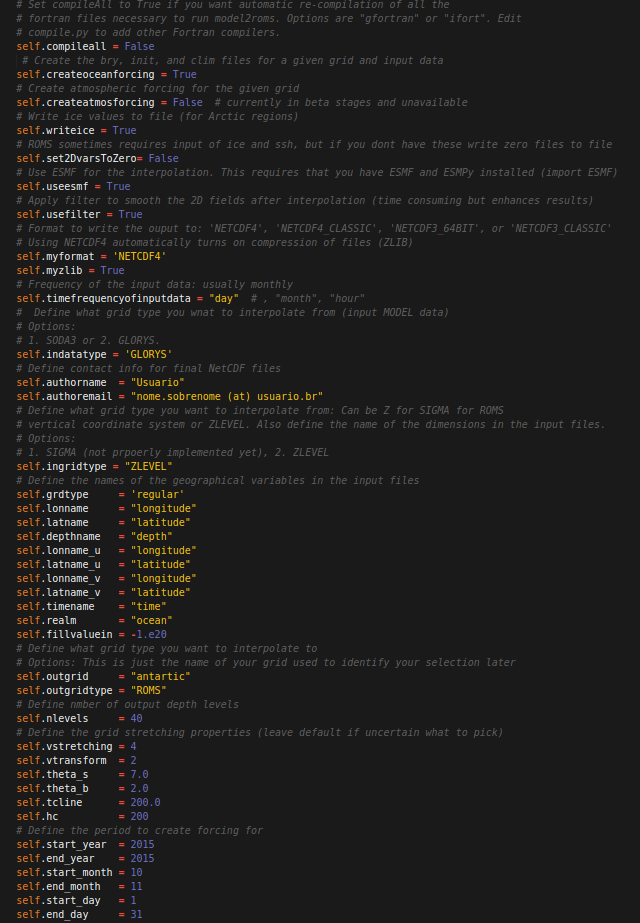
\includegraphics[width=0.5\textwidth]{m2roptions.png}
    \caption{Screenshot of the \textit{configM2R.py} code.}
    \label{m2roptions}
\end{figure}
\bigskip

Run \textit{model2roms} with the command:
\bigskip

\begin{bashcode}
ipython runM2R.py
\end{bashcode}
\bigskip

At the end, the initial, boundary and climatological files will be created, which should be added to your project folder, in the Kerana cluster.
\bigskip
   
